% Das Management Summary richtet sich in der Praxis an die "Chefs des Chefs", d.
% h. an die Vorgesetzten des Auftraggebers (diese sind in der Regel keine
% Fachspezialisten).
% Die Sprache soll knapp, klar und stark untergliedert sein.
% Zu verwenden ist folgenden Gliederung:
% - Ausgangslage - Vorgehen, Technologien - Ergebnisse - Ausblick (optional)

\chapter*{Management Summary}\addcontentsline{toc}{chapter}{Management Summary}

\paragraph{Ausgangslage}~\\
In der Verkehrs- und der Raumplanung werden ÖV-Güteklassen für die Beurteilung eines Standortes bezüglich der Erschliessung mit dem öffentlichen Verkehr verwendet.
Durch diese können Entscheidungen bezüglich der Entwicklung eines Standortes getroffen werden.
So macht es Sinn an bereits an gut erschlossenen Standorten zu verdichten und nicht neues Bauland zu erschliessen, um nachträglich die ÖV-Infrastruktur hochziehen zu müssen.
Der Nutzen der ÖV-Güteklassen beschränkt sich nicht auf Verkehrs- und Raumplaner.
Privatpersonen können ebenso bei der Wohnungs- wie auch der Wohnungssuche Gebrauch davon machen.
Ein Wohnort mit guter ÖV-Anbindung ist in Zeiten erhöhter Mobilität von hohem Stellenwert.

Die Methodik zur Erhebung von ÖV-Güteklassen wurde erstmals 1993 in einer inzwischen ersetzten Schweizer Norm festgelegt.
Auf Grundlagen dieser hat das Bundesamt für Raumentwicklung (ARE), sowie verschiedene Kantone Berechnungsmethodiken entwickelt.
Diese weichen unterschiedlich stark von der Norm ab.

Diese Berechnungsmethodiken sind für die heutigen technischen Möglichkeiten überholt.
So wird unteranderem das Einzugsgebiet wie in Abbildung \ref{fig:grid_based_approach} sichtbar mit Luftlinien berechnet. 

\begin{figure}[ht]
    \centering
    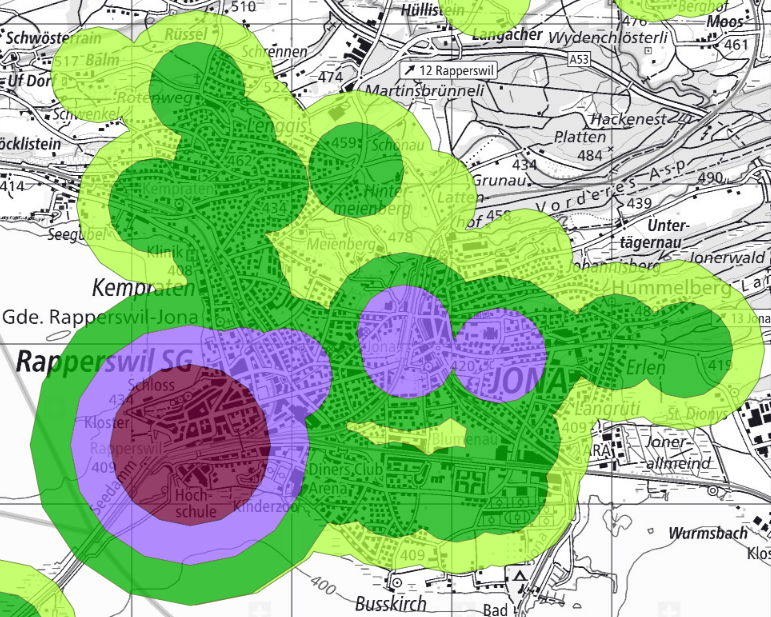
\includegraphics[width=0.8\linewidth]{start/img/air_line_ARE.png}
    \caption[Luftlinie bei Einzugsgebieten]{Luftlinie bei Einzugsgebieten}
    \label{fig:air_line_ARE}
\end{figure}

Der Topografie wird in den aktuellen Lösungen nur wage Beachtung geschenkt.
So ist nicht klar, in welchem Mass eine anspruchsvollere Topografie zu buche schlägt.

\paragraph{Ziele, Vorgehen und Technologien}~\\
Im Kontext der Arbeit ÖV-Güteklassen 2018 wird in einem ersten Schritt eine neue Spezifikation entwickelt, welche auf dem Fundament der bestehenden Lösungen aufbaut, die Probleme dieser aufgreift und den aktuell technischen Möglichkeiten angleicht.
So soll unteranderem die genaue Wegführung beim Berechnung des Einzugsgebiet berücksichtigt und der Topografie Rechnung getragen werden.
Die theoretisch erarbeitete Spezifikation \emph{ÖV-Güteklassen 2018} wird in 

%TODO

\paragraph{Ergebnisse}~\\

%TODO

\paragraph{Ausblick}~\\
In der vorliegenden Arbeit wurde beim Berechnen der Erreichbarkeit der Fokus auf eine route-basierte Methode, namentlich Isochronen, gelegt.
Ein weiterer spannender Ansatz, welcher in Betracht gezogen werden kann, ist ein grid- beziehungsweise raster-basierter Ansatz.
In Abbildung \ref{fig:grid_based_approach} wurde dieser Ansatz für die Berechnung der Reisezeit zu einer Haltestelle eines Fussgängers verwendet.
Dabei wird über ein Gebiet ein Raster gelegt, den Rastern eine Kategorie mit zugehörigen Kosten zugewiesen.
Bei den Kosten handelt es sich im abgebildeten Fall um die Überwindungsgeschwindigkeit des jeweiligen Rasters.
So erhält ein Raster mit einem Hinderniss die Geschwindigkeit 0 km/h und eine Grünfläche 2 km/h.
Dies hat unteranderem den Vorteil, dass man nicht direkt vom Routing-Netzwerk abhängig ist und auch offene Flächen wie Plätze und Grünflächen einbezogen werden.
Es lässt sich darüber streiten, ob alle Grünflächen von Fussgänger begehbar sind.
Ebenfalls lassen sich offene Fläche für die bestehende Lösung durch eine Vorverarbeitung des Routing-Netzwerk beispielsweise durch \emph{PlazaRoute}~\cite{plaza_route} ins Routing-Netzwerk integrieren.

\begin{figure}[ht]
    \centering
    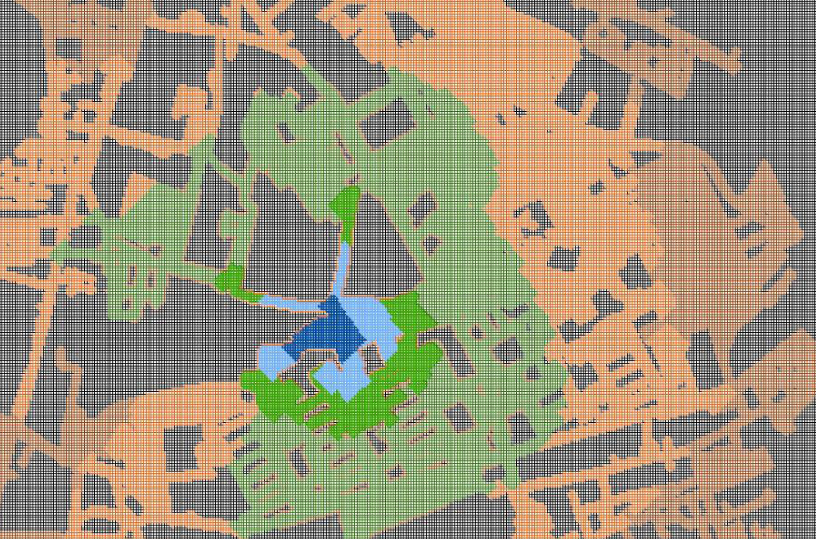
\includegraphics[width=0.8\linewidth]{start/img/grid_based_approach.png}
    \caption[Grid- beziehungsweise raster-basierter Ansatz]{Grid- beziehungsweise raster-basierter Ansatz~\cite{pedestrian_accessibility_planning}}
    \label{fig:grid_based_approach}
\end{figure}
%TODO